\section{Experiments and Results Analysis} 
\label{sec:exp-results}

\subsection{Implementation Details}
\label{sec:exp-implementation}

\begin{figure}[htbp]
    \centering
    \begin{minipage}{0.45\textwidth}
        \centering
        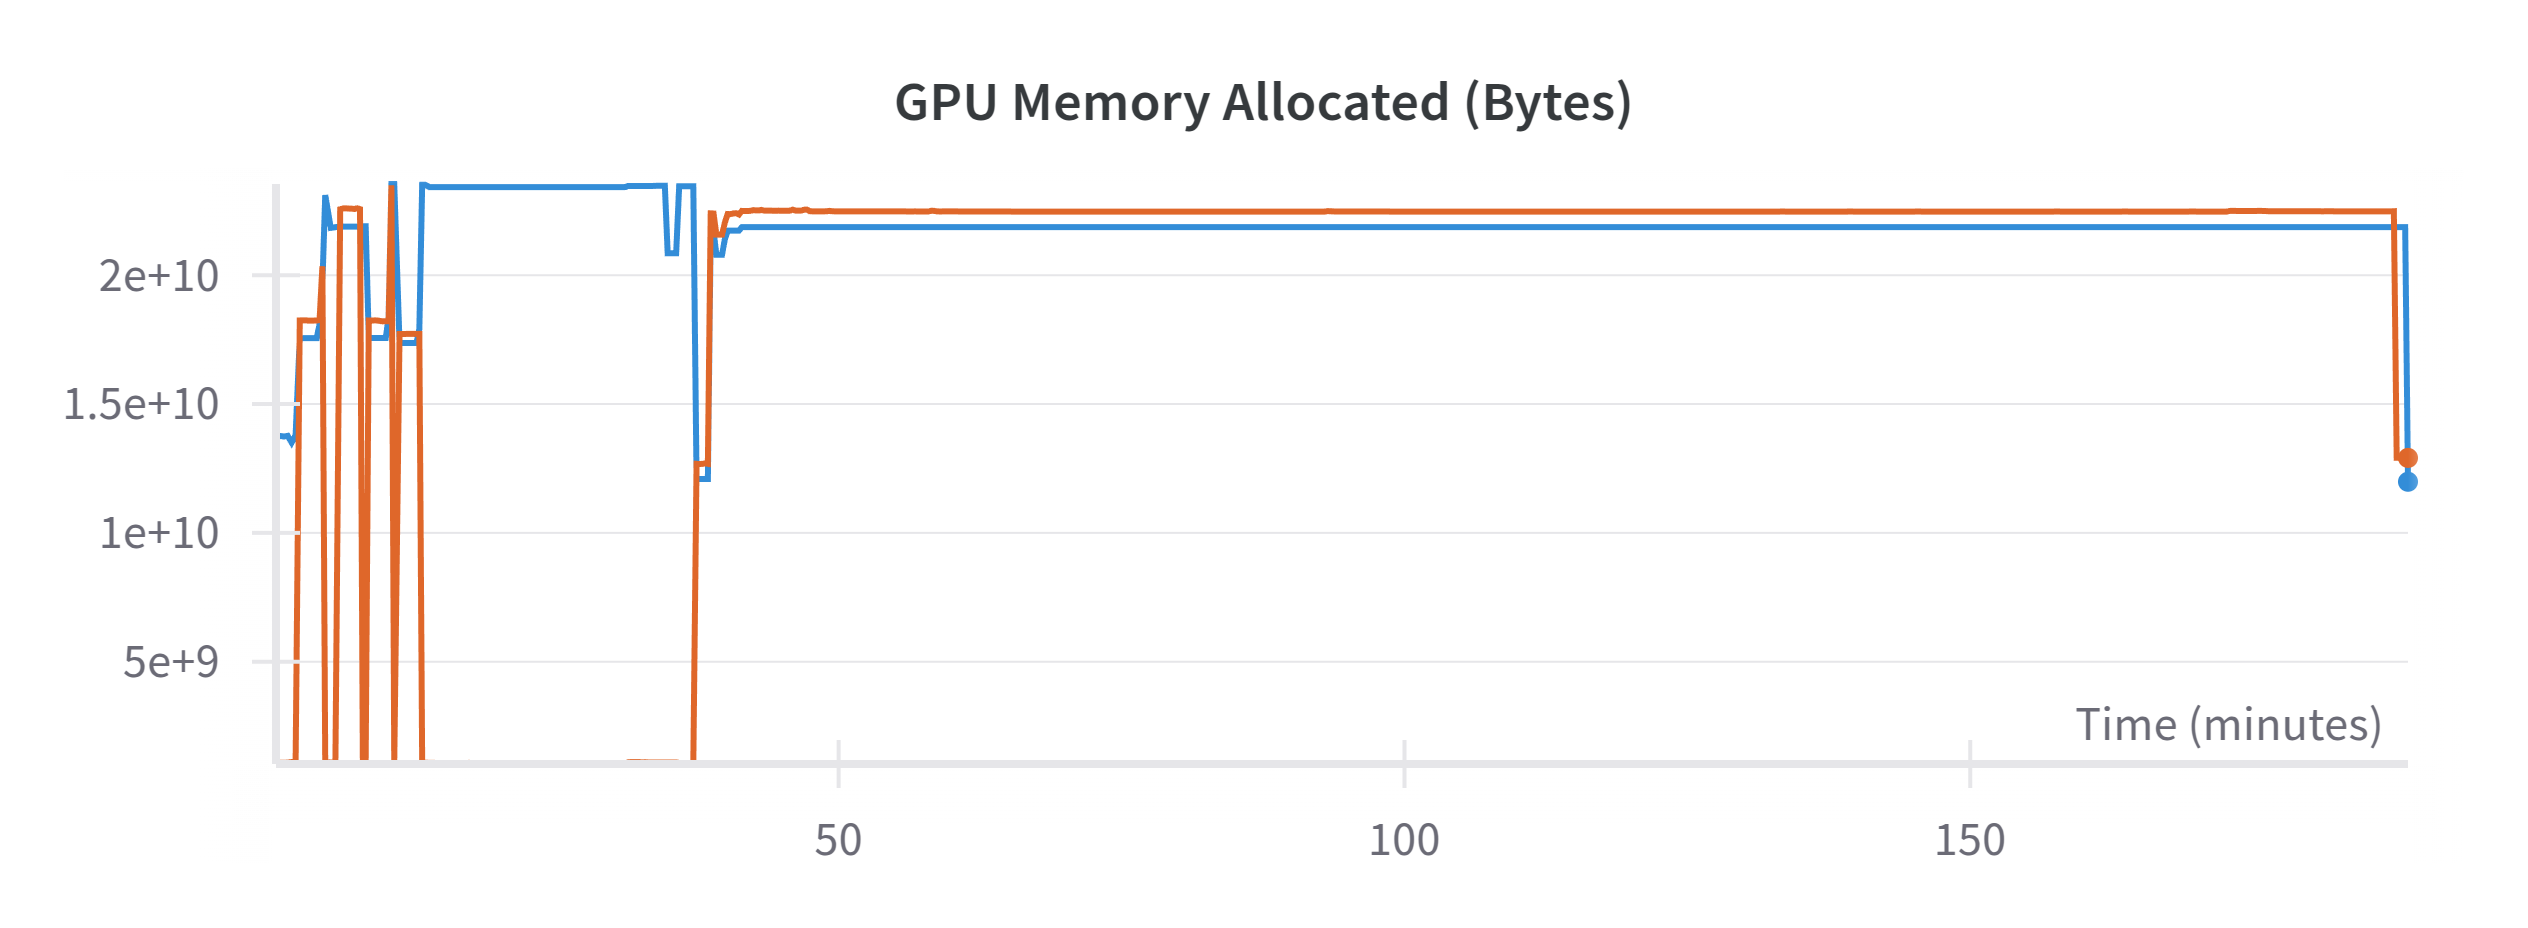
\includegraphics[width=\textwidth]{figs/gpu_mem.png}  
        \label{fig:gpu_mem}
    \end{minipage}\hfill
    \begin{minipage}{0.45\textwidth}
        \centering
        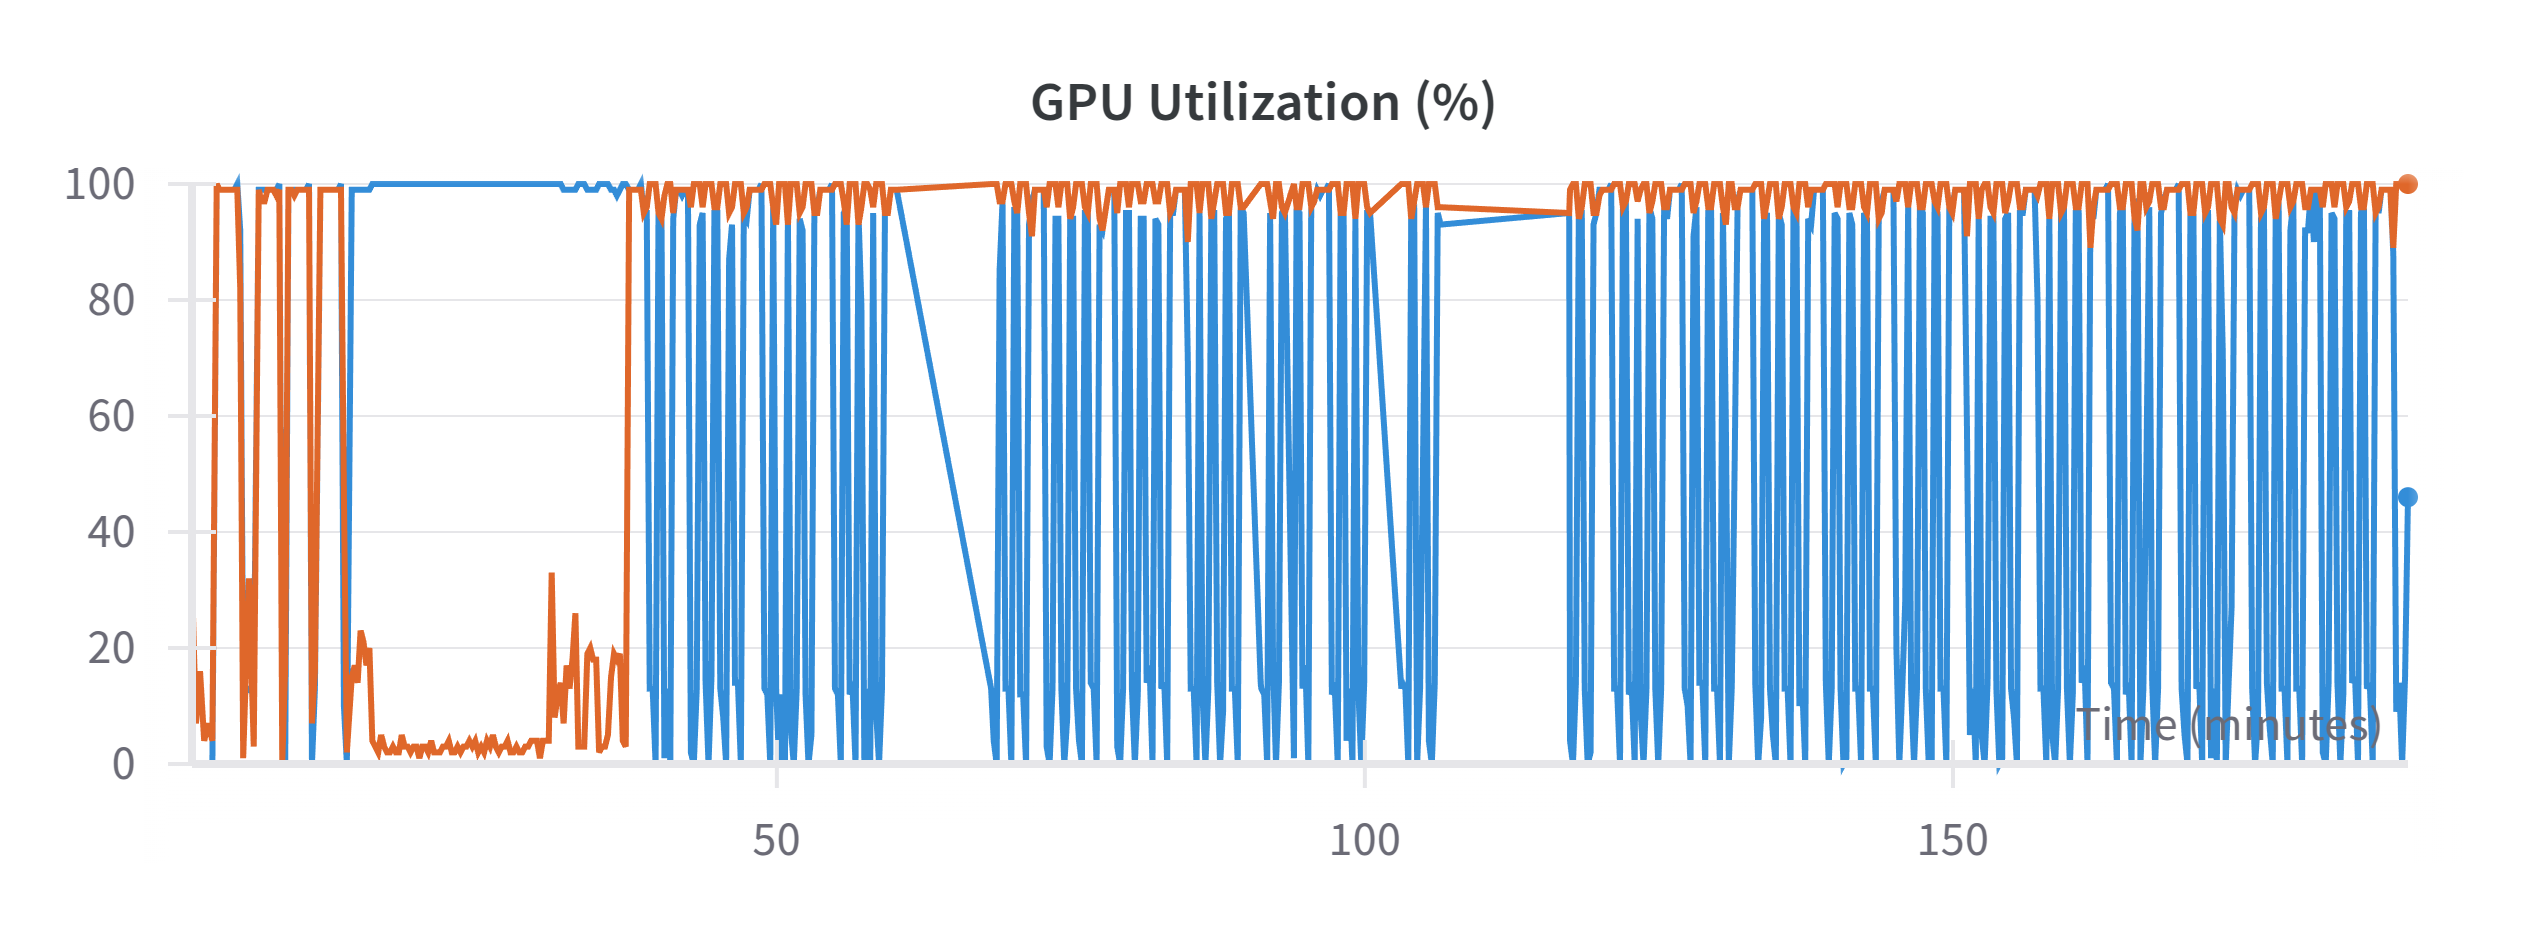
\includegraphics[width=\textwidth]{figs/gpu_util.png}  
        \label{fig:gpu_util}
    \end{minipage}
    \caption{GPU Memory and Utilization}
    \label{fig:gpu_mem_util}
\end{figure}

Training was conducted on a dual-GPU system with \textit{two NVIDIA RTX 2080 Ti (22GB VRAM each)}
    in a distributed data-parallel (DDP) configuration, providing a total effective memory of 44 GB.
The framework leveraged PyTorch Lightning for distributed training and checkpoint management
    (\codeblock{lightning.yaml}), with the hyperparameters:
\begin{itemize}
    \item \texttt{Batch Size}: 
    A per-GPU batch size of 2 with gradient accumulation over 8 steps 
        (effective batch size = 16) to balance memory constraints and training stability.
    \item \texttt{Learning Rate}: 
    Initialized at \textit{1e-4} with the \textit{AdamW} optimizer configuration in \codeblock{train.yaml}.
    \item \texttt{Training Duration}: 
    100 epochs with early stopping based on validation loss plateaus.
\end{itemize}

\begin{figure}[htbp]
    \centering
    \begin{minipage}{0.45\textwidth}
        \centering
        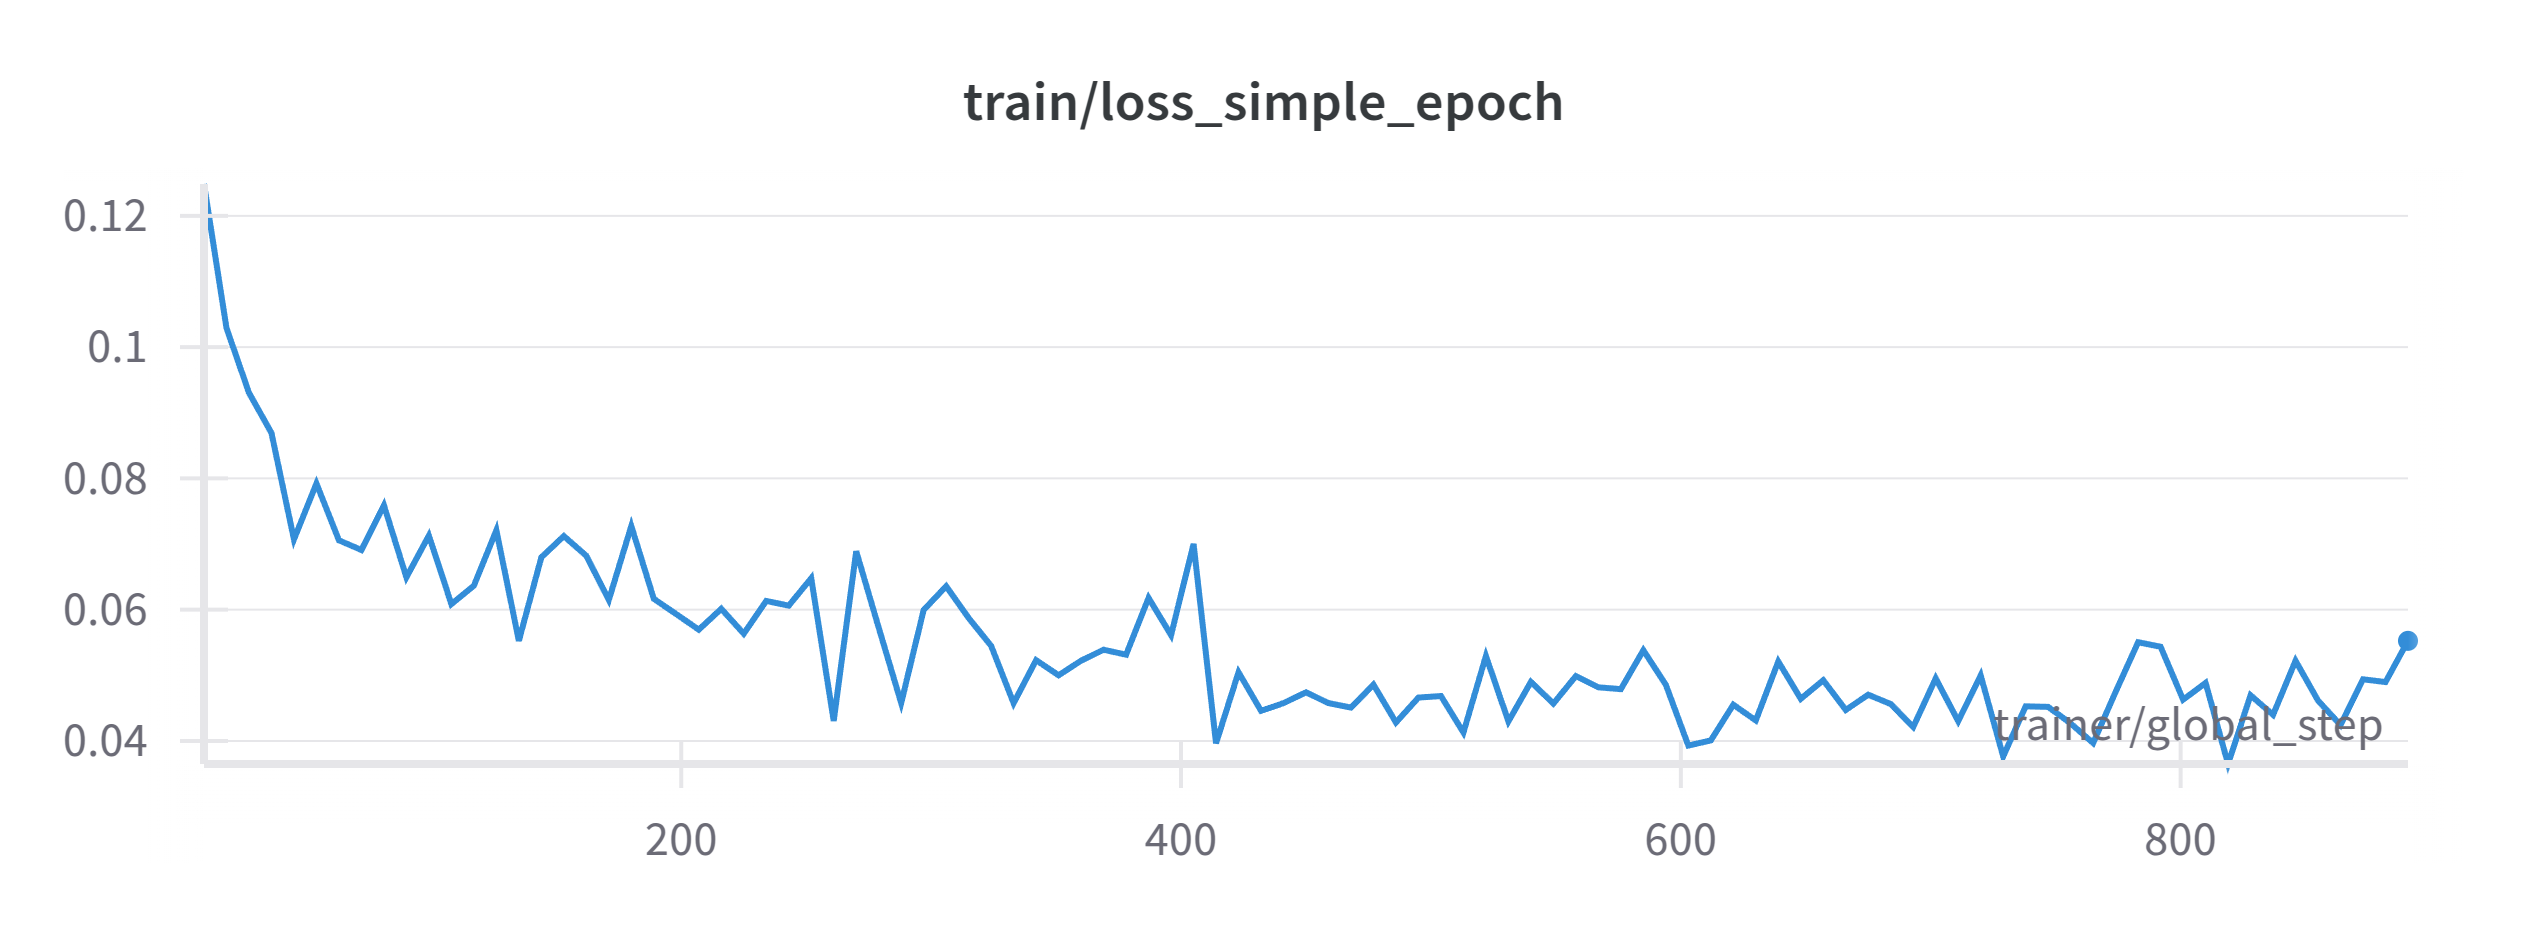
\includegraphics[width=\textwidth]{figs/train_loss.png}  
        \label{fig:train_loss}
    \end{minipage}\hfill
    \begin{minipage}{0.45\textwidth}
        \centering
        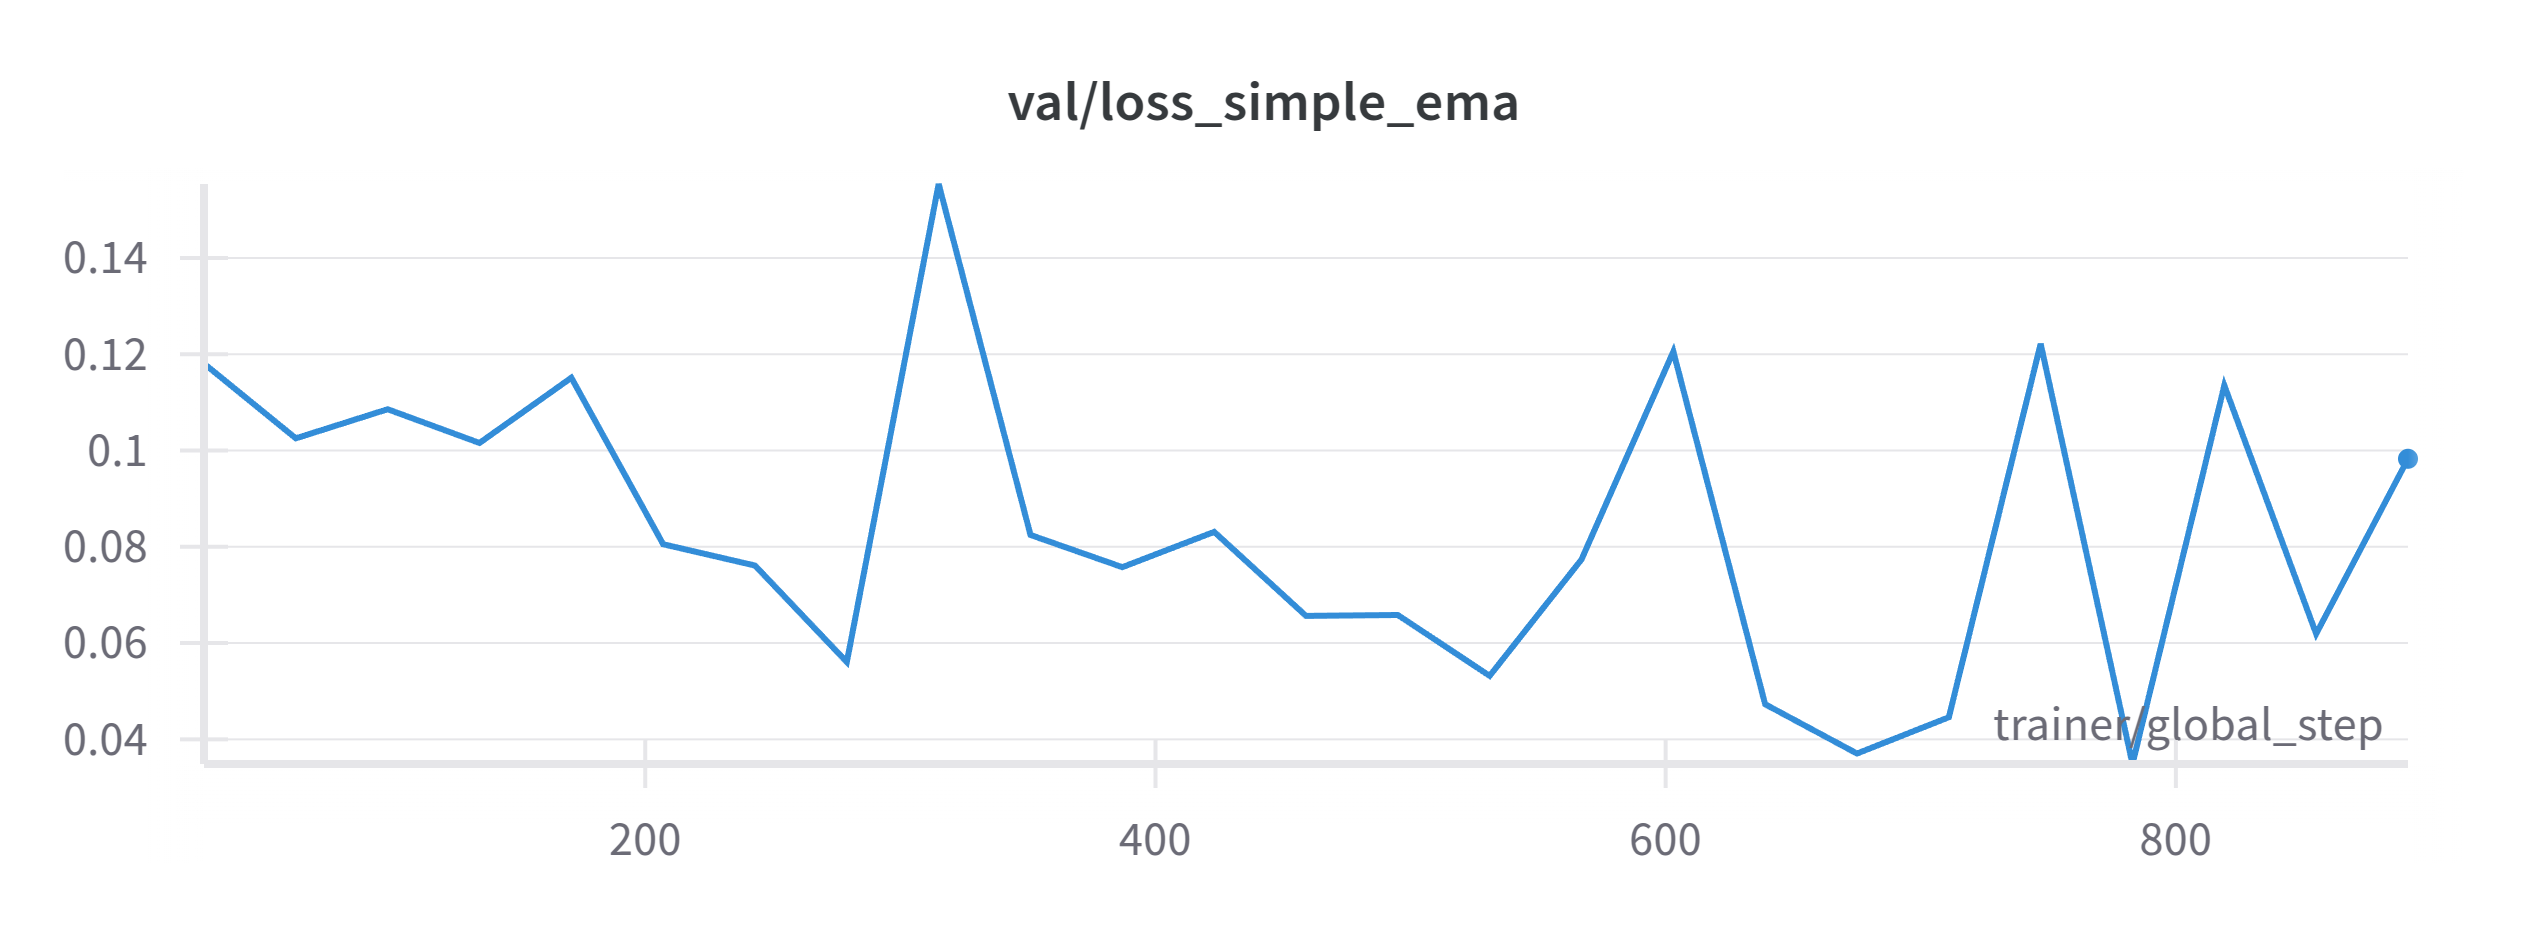
\includegraphics[width=\textwidth]{figs/val_loss.png}  
        \label{fig:validation_loss}
    \end{minipage}
    \caption{Training and Validation Loss Curves}
    \label{fig:loss_curves}
\end{figure}


\subsection{Evaluation Metrics}
\label{sec:exp-metrics}

\textbf{SSIM (Structural Similarity Index):} \\
\noindent
Quantifies structural consistency between generated and ground-truth frames by comparing luminance, contrast, and structure. 
Higher values for better perceptual alignment.

\noindent
\textbf{PSNR (Peak Signal-to-Noise Ratio):}\\
\noindent
Measures pixel-level reconstruction fidelity by computing the logarithmic ratio of peak signal power to noise. 
Higher values denote lower distortion.

\subsection{Results and Analysis}
\label{sec:exp-results-analysis}

The model achieves strong generalization across tasks:~\ref{tab:performance_metrics}

\begin{table}
    \centering
    \begin{tabular}{@{}lcc@{}}
        \toprule
        \textbf{Task} & \textbf{SSIM} & \textbf{PSNR (dB)} \\
        \midrule
        \texttt{block\_hammer\_beat} & 0.97 & 38.5 \\
        \texttt{block\_handover} & 0.98 & 40.1 \\
        \texttt{block\_stack\_easy} & 0.95 & 37.8 \\
        \bottomrule
    \end{tabular}
    \caption{Performance Metrics for Different Tasks}
    \label{tab:performance_metrics}
\end{table}

The \textit{block\_handover} task (SSIM=0.98, PSNR=40.1 dB) demonstrates superior performance 
    due to its deterministic motion patterns, 
whereas \textit{blocks\_stack\_easy} (SSIM=0.95) shows slightly lower metrics, 
    likely due to the stochasticity in block stacking dynamics.
The final validation loss stabilizes at 0.038 (see \codeblock{wandb-summary.json}), 
    indicating robust convergence despite limited data.
While no direct baseline comparison is provided, 
    the results highlights the efficacy of task-specific fine-tuning.

\subsection{Visualization}
\label{sec:exp-visualization}

\begin{figure}[htbp]
    \centering
    \begin{minipage}{0.45\textwidth}
        \centering
        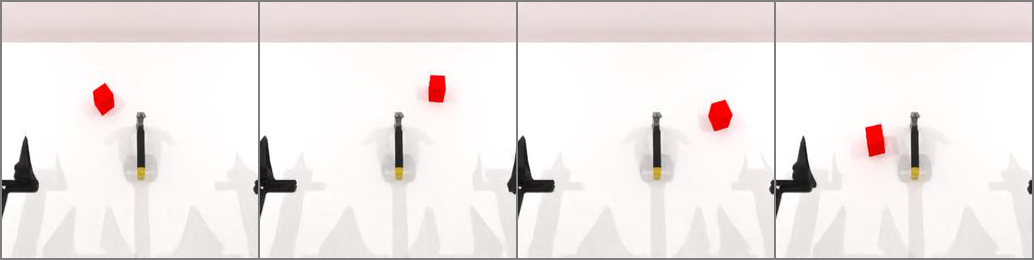
\includegraphics[width=\textwidth]{figs/val_before.png}
        \subcaption{Original Frame}  
    \end{minipage}\hfill
    \begin{minipage}{0.45\textwidth}
        \centering
        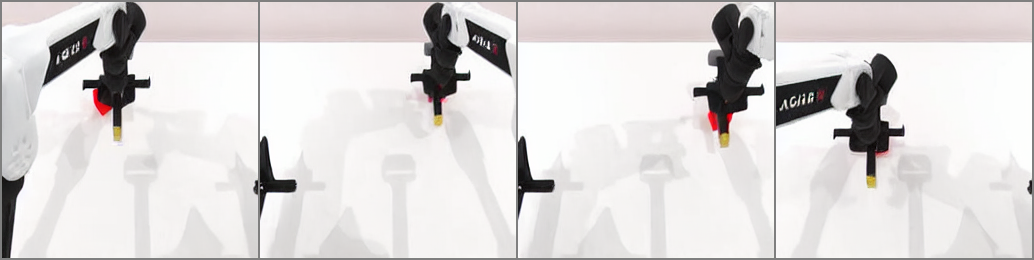
\includegraphics[width=\textwidth]{figs/val_before-vq.png}  
        \subcaption{Generated Frame}
    \end{minipage}\hfill
    \begin{minipage}{0.45\textwidth}
        \centering
        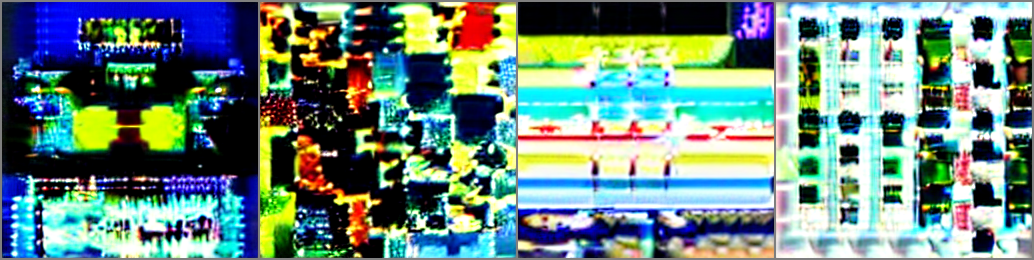
\includegraphics[width=\textwidth]{figs/val_after-gen.png}  
        \subcaption{VQ-encoded Frame}
    \end{minipage}
    \caption{Validation Frame Example on \textit{block\_hammer\_beat} Task}
    \label{fig:val_example}
\end{figure}

We visualize predictions for all three tasks in a 3$\times$3 grid (Figure ~\ref{fig:visual_example}), 
    contrasting input frames, generated frames, and ground-truth sequences. Key findings include:

\begin{itemize}
    \item \textbf{High-Fidelity Reconstruction:} 
    Generated frames preserve fine-grained details (e.g., hammer trajectory in \textit{block\_hammer\_beat}) 
        and maintain the structural integrity (e.g., block edges in \textit{block\_handover}).
    \item \textbf{Instruction Alignment:} 
    The model accurately interprets textual commands (e.g., \textit{"stack blocks"} results in vertically aligned blocks),
        demonstrating effective integration of language and visual modalities.
    \item \textbf{Limitations:} 
    Minor artifacts (blurring at object edges) occur in high-motion scenarios (e.g., rapid handover actions), 
        likely due to the diffusion model iterative sampling process with limited training data.
\end{itemize}

\noindent
\textbf{Weights and Biases Training Dynamics:}
\url{https://wandb.ai/jim_choi-chinese-university-of-hong-kong-shenzhen/uncategorized/runs/train_default/overview}

\begin{figure}[htbp]
    \centering
    \begin{minipage}{0.45\textwidth}
        \centering
        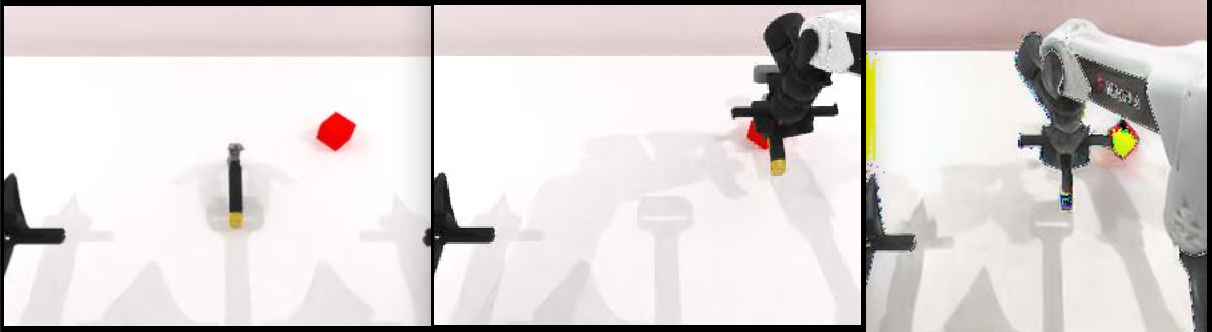
\includegraphics[width=\textwidth]{figs/block_hammer_beat.png}
        \subcaption{Block Hammer Beat}  
    \end{minipage}\hfill
    \begin{minipage}{0.45\textwidth}
        \centering
        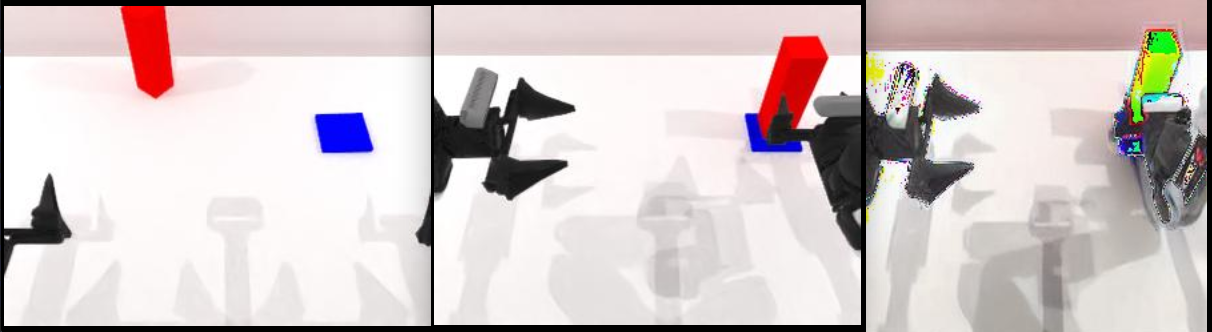
\includegraphics[width=\textwidth]{figs/block_handover.png}  
        \subcaption{Block Handover}
    \end{minipage}\hfill
    \begin{minipage}{0.45\textwidth}
        \centering
        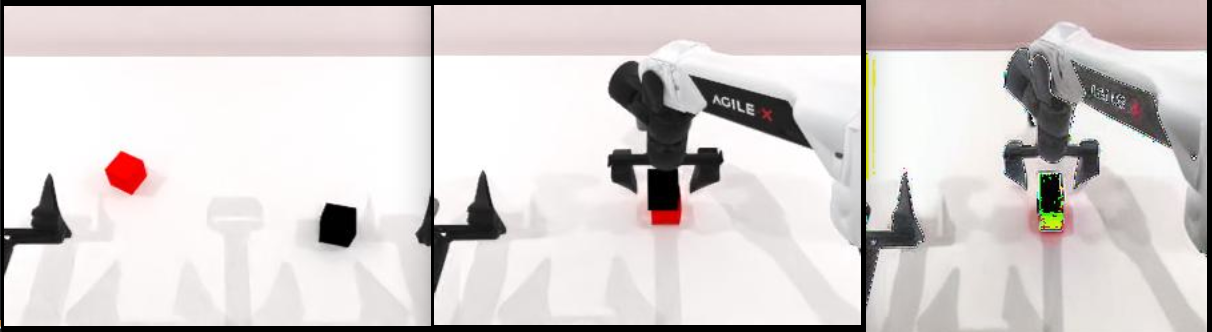
\includegraphics[width=\textwidth]{figs/block_stack_easy.png}  
        \subcaption{Block Stack Easy}
    \end{minipage}
    \caption{Visualization Frame Examples on Different Tasks}
    \label{fig:visual_example}
\end{figure}